%-*-latex-*-
\sectionthree{Sparse long integer}
\begin{python0}
from solutions import *; clear()
\end{python0}

\begin{ex}
What if there are lots of zeroes in your integer?
Say the integer is
\[
\text{\texttt{50000061000200004}}
\]
Assume that an \verb!int! 4 bytes (i.e., 32 bits),
%\sidebar{ANSWER. $17 \cdot 4. n \cdot 4$.}
how many bytes are used when you model the above integer (with 17 digits)
an array of \verb!int!s? What if there are $n$ digits?

Now the above integer is the same as
\[
5 \cdot 10^{16} + 6 \cdot 10^{10} + 1 \cdot 10^9 + 2 \cdot 10^5
    + 4 \cdot 10^0
\]
So we can have (doubly linked) nodes where each nonzero term corresponds to
one node, storing the
exponent (of 10) and the digit of the term in the node:

\begin{center}
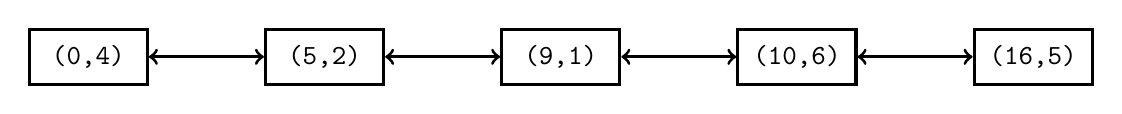
\begin{tikzpicture}

\draw (0.75, 0.35)
  node[draw, line width=0.04cm, , color=black,
       rounded corners=0cm, inner sep=0cm] {

\begin{minipage}[t][0.7cm]{1.5cm}
\mbox{}

\end{minipage}

};\draw (0.75, 0.35) node[color=black] {{\texttt{(0,4)}}};
\draw (3.75, 0.35)
  node[draw, line width=0.04cm, , color=black,
       rounded corners=0cm, inner sep=0cm] {

\begin{minipage}[t][0.7cm]{1.5cm}
\mbox{}

\end{minipage}

};\draw (3.75, 0.35) node[color=black] {{\texttt{(5,2)}}};
\draw (6.75, 0.35)
  node[draw, line width=0.04cm, , color=black,
       rounded corners=0cm, inner sep=0cm] {

\begin{minipage}[t][0.7cm]{1.5cm}
\mbox{}

\end{minipage}

};\draw (6.75, 0.35) node[color=black] {{\texttt{(9,1)}}};
\draw (9.75, 0.35)
  node[draw, line width=0.04cm, , color=black,
       rounded corners=0cm, inner sep=0cm] {

\begin{minipage}[t][0.7cm]{1.5cm}
\mbox{}

\end{minipage}

};\draw (9.75, 0.35) node[color=black] {{\texttt{(10,6)}}};
\draw (12.75, 0.35)
  node[draw, line width=0.04cm, , color=black,
       rounded corners=0cm, inner sep=0cm] {

\begin{minipage}[t][0.7cm]{1.5cm}
\mbox{}

\end{minipage}

};\draw (12.75, 0.35) node[color=black] {{\texttt{(16,5)}}};\draw[line width=0.04cm,black,<->] (1.52,0.35) to  (2.98,0.35);
\draw[line width=0.04cm,black,<->] (4.52,0.35) to  (5.98,0.35);
\draw[line width=0.04cm,black,<->] (7.52,0.35) to  (8.98,0.35);
\draw[line width=0.04cm,black,<->] (10.52,0.35) to  (11.98,0.35);
\end{tikzpicture}

\end{center}


\qed
\end{ex}
Assume that an \verb!int! and a pointer uses 4 bytes (i.e., 32 bits),
%\sidebar{ANSWER: $5 \cdot 4 \cdot 4$. $rn \cdot 4 \cdot 4$.}
how many bytes are used when you model the above integer (with 17 digits)
with this new method? What if there are $n$ digits bit but only $rn$
($r < 1$) are nonzero?

Therefore if $r$ is the fraction of nonzero terms in a long integer
with $n$ digits, then the second method uses less memory if
\[
rn \cdot 4 \cdot 4 < n \cdot 4
\]
i.e.,
\[
r < 1/4
\]
In particular if you want to store
\[
1 \times 10^{100}
\]
The second method uses 16 bytes while the
first method uses ... $101 \cdot 4 = 404$ bytes ... ouch.
The second method is way better.

\begin{ex}
Implement a polynomial class using the above idea.
In the case of polynomials used in cryptography
and signal processing (example: error correction codes),
you \textit{do} see a lot of cases where most of the coefficients are
zero.
For instance the binary polynomial
\[
x^{571} + x^{10} + x^5 + x^2 + 1
\]
is recommended for use in elliptic curve crygtography.
(See \url{https://www.secg.org/sec2-v2.pdf}, table 3.)
A binary polynomials is a polynomial where the
coefficients are either 0 or 1.
\qed
\end{ex}
  
